\documentclass[11pt]{book}

\usepackage[a4paper,
top=25mm,bottom=10mm,left=32mm,
right=32mm,marginparwidth=1.75cm]{geometry}

\usepackage[utf8]{inputenc}
\usepackage[T1]{fontenc}
\usepackage{helvet}
\renewcommand{\familydefault}{\sfdefault}
\usepackage[english]{babel}
\usepackage{soul}
\usepackage{epsfig}
\usepackage{epstopdf}
\epstopdfsetup{update}
\usepackage{graphicx}
\usepackage{float}
\usepackage{array}
\newcolumntype{L}[1]{>{\raggedright\arraybackslash}m{#1}}

\usepackage{amsmath,amssymb,amstext}

\usepackage{titlesec}
\setcounter{secnumdepth}{0}
\titleformat{\section}
{\normalfont\fontsize{11pt}{12pt}\selectfont
\bfseries\filright}{}{0em}{}
%
\titlespacing{\section}
{0pc}{*3.2}{*1.0}[0pc]

\titleformat{\subsection}
{\normalfont\fontsize{11pt}{12pt}\selectfont
\bfseries\filright}{}{0.5em}{}
%
\titlespacing{\subsection}
{0pc}{*3.2}{*0.2}[0pc]

\usepackage{pifont}
\newcommand{\cmark}{\ding{51}}%
\newcommand{\xmark}{\ding{55}}
\usepackage{makecell}
\usepackage{arydshln}
\usepackage{enumitem}
\setlist[itemize]{labelindent=*, leftmargin=*, itemsep=-3pt,
label={\makebox[0pt][l]{$\square$}\raisebox{.15ex}{\hspace{0.1em}$\checkmark$}}}

\newcommand{\nocheck}{\mbox{\makebox[0pt][l]{$\square$}\raisebox{.15ex}{\hspace{0.1em}{$\phantom{\checkmark}$}}}}
\parindent=0mm
\pagestyle{empty}

\begin{document}


Form A

\section{Expansion of Hong Kong International Airport into a Three-Runway System}

Marine Travel Routes and Management Plan for High Speed Ferries of SkyPier

\subsection{\ul{Environmental Audit Checking Record}}

{\renewcommand{\arraystretch}{1.4}
\begin{table}[htb]
\fontsize{11pt}{15pt}\selectfont
\begin{tabular}{|>{\raggedright}p{39mm}|
p{98mm}<{\raggedright}|}\hline
%%
Reference Plan: & Marine Travel Routes and Management Plan for High Speed Ferries of SkyPier (EP Condition 2.10)
\\[0.5mm] \hline
Monitoring Data: & Ferry movement data collected in the period between
\newline
\ul{%(Period)s}
\\[1.0mm] \hline
Information and Data Checked: &
\begin{minipage}[t]{110mm}
\begin{itemize}
\item Automatic Identification System (AIS) Data
\item Daily SkyPier HSF movements
\item Record of potential deviations
\item Response provided by the ferry operators
\end{itemize}
\end{minipage}
\\[0.1mm]\hline
Comments and Observations: &
The deviation of implementation of SkyPier HSF plan was checked. %(No.of Cases)s  issued by AAHK to ferry operators related to potential speeding across the SCZ, not travelling through the gate access points and insufficient AIS data. The audit results from %(Period)s will be included in the
%(No. of EM&A Report)s\textsuperscript{%(Subscript)s} Monthly EM\&A Report.
 \\ \hline
\end{tabular}
\end{table}
}


{\fontsize{10pt}{12pt}\selectfont
\begin{tabular}{:L{23mm}:L{35mm}:L{35mm}:L{35mm}:}
\hdashline
\Gape[14pt]{}& \makecell[l]{ET Leader /\\[2mm]
ET's Representative} &
\makecell[l]{IEC/ \\[2mm]
IEC's Representative} &
\makecell[l]{PM /\\[2mm]
PM's Representative} \\ \hline
Signature &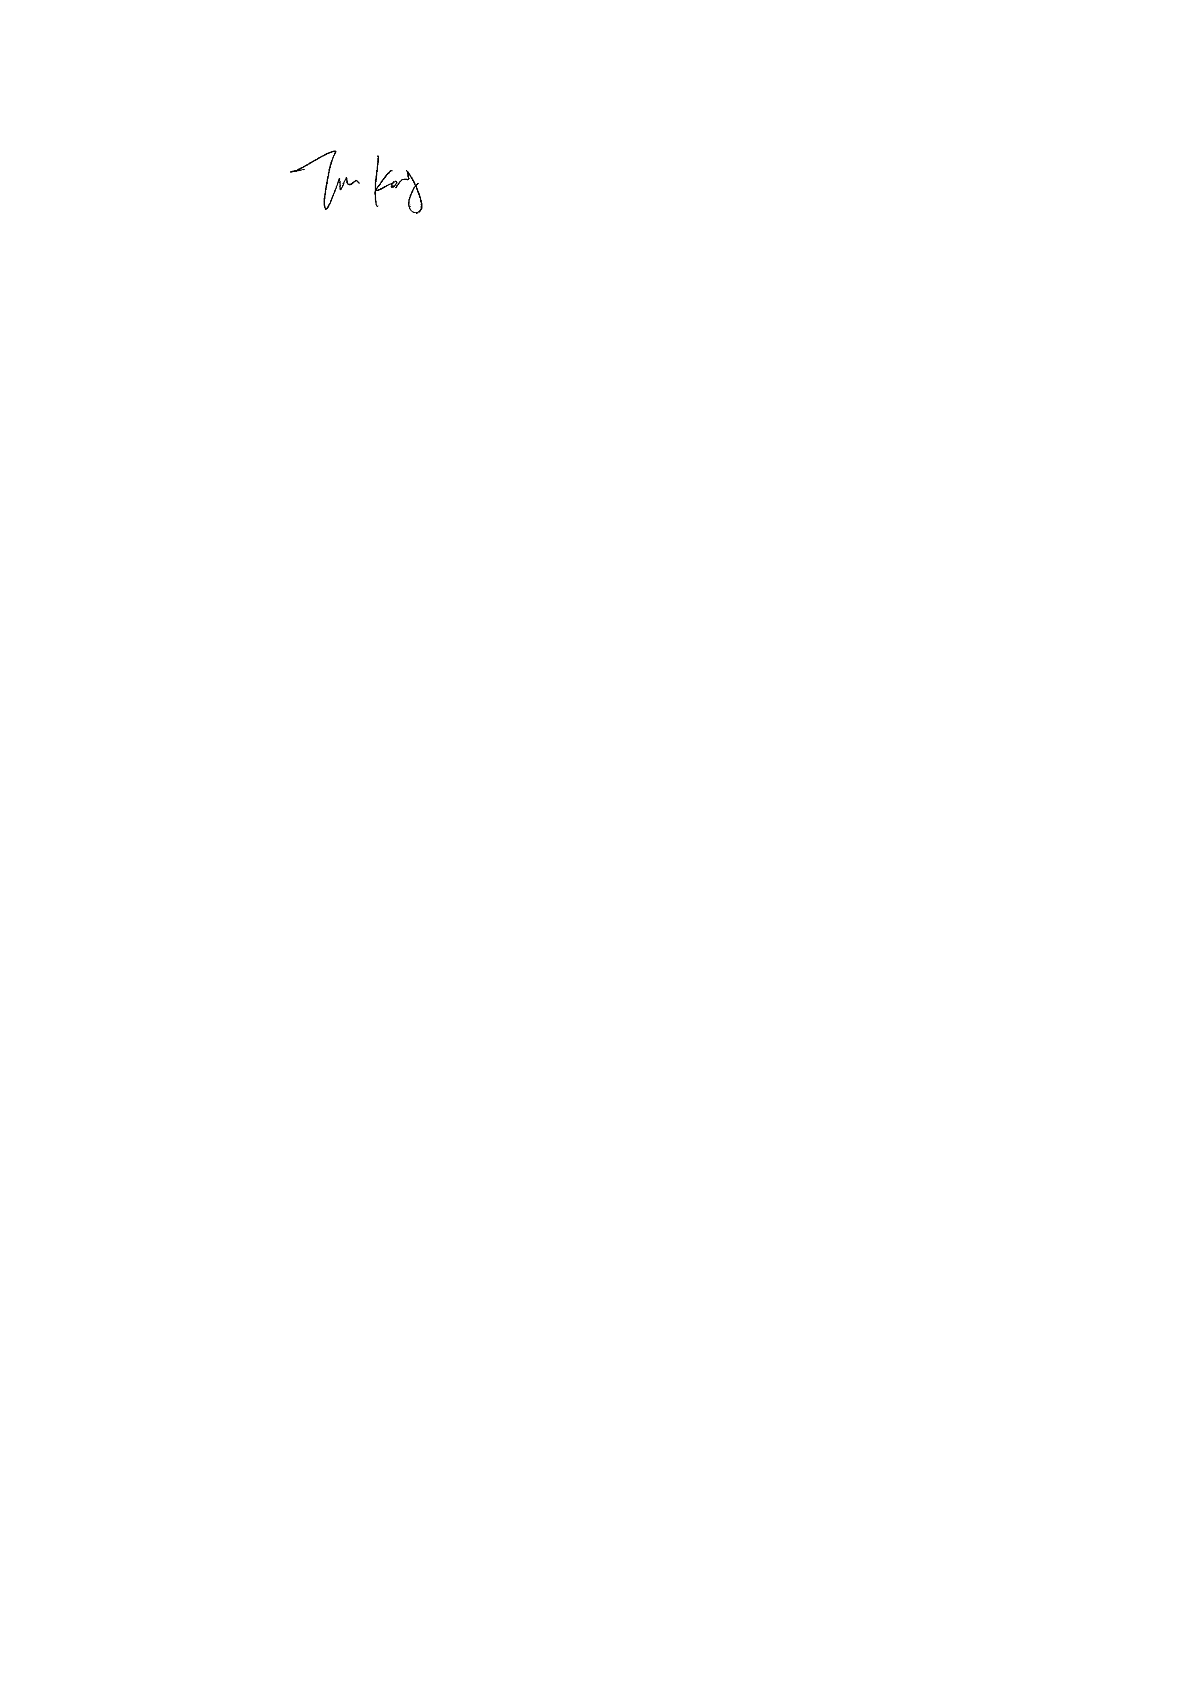
\includegraphics[scale=1.0]{sig1.pdf}
&  &  \\ \hdashline
Name & Terence Kong &  &
\Gape[10pt]{}
\\\hdashline
\end{tabular}
}

\end{document}
